% Wei-Jin Huang -- English research CV, weijincv v2
% Build from this directory:
%   latexmk -xelatex -interaction=nonstopmode -halt-on-error \
%     -jobname=wei_jin_huang_cv_weijincv_v2_en cv.tex
\documentclass[10pt,a4paper]{article}

\usepackage[left=0.9cm,right=0.9cm,top=0.35cm,bottom=0.35cm]{geometry}
\usepackage{fontspec}
\usepackage{microtype}
\usepackage{fontawesome5}
\usepackage{enumitem}
\usepackage{graphicx}
\usepackage{array}
\usepackage{tabularx}
\usepackage{xcolor}
\usepackage[hidelinks]{hyperref}

\hypersetup{
  pdftitle={Wei-Jin Huang -- Curriculum Vitae},
  pdfauthor={Wei-Jin Huang}
}
\pagestyle{empty}
\setlength{\parindent}{0pt}
\setlength{\parskip}{1.5pt}
\setlength{\emergencystretch}{1em}
\linespread{1.04}
\sloppy

\definecolor{muted}{HTML}{4A4A4A}

% Icon, title, and full-width rule: retained from the collaborator's visual system.
\newcommand{\cvsection}[2]{%
  \vspace{5pt}%
  {\large\bfseries #1\hspace{0.5em}#2}\par
  \vspace{1pt}%
  \hrule width \linewidth height 0.6pt
  \vspace{3pt}%
}

\newcommand{\papertitle}[2]{%
  \if\relax\detokenize{#2}\relax
    \textbf{#1}%
  \else
    \href{#2}{\textbf{#1}}%
  \fi
}

% title / authors / full venue (abbreviation and year) / overview / URL
\newcommand{\paper}[5]{%
  \papertitle{#1}{#5}\par
  {\small\bfseries #3}\par
  {\color{muted}#2}\par
  \begin{itemize}[leftmargin=1.2em,topsep=1pt,itemsep=1pt,parsep=0pt,partopsep=0pt]
    \item #4
  \end{itemize}
  \vspace{1pt}%
}

% Education detail rows: equal side columns place the middle detail on the page center.
\newcommand{\edudetail}[3]{%
  \noindent
  \begin{tabularx}{\linewidth}{@{}>{\raggedright\arraybackslash}p{0.24\linewidth}@{}>{\centering\arraybackslash}X@{}>{\raggedleft\arraybackslash}p{0.24\linewidth}@{}}%
    #1 & #2 & #3
  \end{tabularx}\par
}

\begin{document}

% ============================ HEADER ========================================
\begin{center}
  \begin{minipage}[c]{0.12\linewidth}
    
\includegraphics[width=1.9cm]{figs/logo-sysu.png}
  \end{minipage}%
  \begin{minipage}[c]{0.74\linewidth}
    \centering
    {\LARGE\bfseries Wei-Jin Huang}\\[3pt]
    {\footnotesize Ph.D. Student in Computer Science and Technology\quad | \quad Sun Yat-sen University\quad Guangzhou, China}\\[3pt]
    \small
    \faEnvelope\ \href{mailto:huangwj235@mail2.sysu.edu.cn}{huangwj235@mail2.sysu.edu.cn}\quad
    \faGlobe\ \href{https://vkgo.github.io/}{vkgo.github.io}\quad
    \faGraduationCap\ \href{https://scholar.google.com/citations?user=jMrU_JYAAAAJ}{Google Scholar}\quad
    \faGithub\ \href{https://github.com/vkgo}{github.com/vkgo}
  \end{minipage}%
  \begin{minipage}[c]{0.12\linewidth}
    \hfill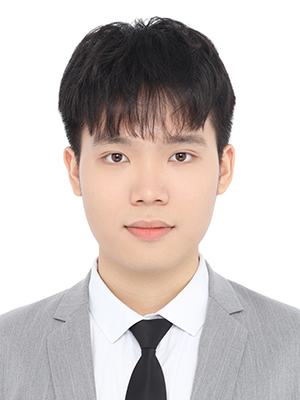
\includegraphics[width=1.9cm]{figs/photo.jpg}
  \end{minipage}
\end{center}

\vspace*{-0.45cm}

% ============================ PROFILE =======================================
\cvsection{\faUser}{Research Profile}
\begin{itemize}[leftmargin=1.2em,topsep=1pt,itemsep=1pt,parsep=0pt,partopsep=0pt]
  \item \textbf{Research Focus:} Ph.D. student at Sun Yat-sen University, advised by Prof. Wei-Shi Zheng, working on \textbf{embodied algorithms for humanoid robots and video action understanding}.
  \item \textbf{Internship Interests:} Combining VLA/WAM models, agentic planning, and continual learning with egocentric human data and robot experience for compositional generalization, rapid adaptation, and failure recovery.
\end{itemize}

% ============================ EDUCATION =====================================
\cvsection{\faGraduationCap}{Education}
\textbf{Sun Yat-sen University (Ph.D.)}\hfill School of Computer Science and Engineering\hfill Sep. 2024 -- Present\\
\edudetail{Computer Science and Technology}{Research: Embodied Intelligence and Computer Vision}{Advisor: Prof. Wei-Shi Zheng (Changjiang Scholar)}

\begin{itemize}[leftmargin=1.2em,topsep=2pt,itemsep=2pt,parsep=0pt,partopsep=0pt]
  \item \textbf{Honors:} Sun Yat-sen University President's Scholarship (top 5\%)
  \item \textbf{Publications:} Multiple first/co-first-author papers at CVPR, ECCV, and ACM MM.
\end{itemize}

\textbf{South China University of Technology (B.E.)}\hfill School of Computer Science and Engineering\hfill Sep. 2020 -- Jul. 2024\\
\edudetail{Network Engineering}{Major Rank: 3/66}{}

\begin{itemize}[leftmargin=1.2em,topsep=1pt,itemsep=1pt,parsep=0pt,partopsep=0pt]
  \item \textbf{Honors:} National Scholarship (1/66), First-Class Tencent Scholarship (1/66)
  \item \textbf{Competitions:} Kaggle H\&M Personalized Fashion Recommendations, Silver (85/2952, 2022); Kaggle G2Net Gravitational Wave Detection, Silver (57/1219, 2021)
\end{itemize}

% ============================ PUBLICATIONS ==================================
\cvsection{\faBook}{Selected Publications}

\paper
  {Beyond Mimicry: Learning Whole-Body Human-Humanoid Interaction from Human-Human Demonstrations}
  {\textcolor{black}{\textbf{Wei-Jin Huang}}, Yue-Yi Zhang, Yi-Lin Wei, Zhi-Wei Xia, Juantao Tan, Yuan-Ming Li, Zhilin Zhao, Wei-Shi Zheng}
  {IEEE/CVF Conference on Computer Vision and Pattern Recognition (CVPR 2026)}
  {\textbf{Overview:} Despite abundant human--human data, high-quality human--humanoid demonstrations are scarce: retargeting breaks key contacts, while standard imitation favors trajectory reproduction over interaction reasoning. PAIR generates executable supervision via contact-preserving, physics-aware retargeting. D-STAR separates \emph{when}/\emph{where}: Phase Attention models stages, Multi-Scale Spatial locates targets, and a diffusion head fuses both into synchronized interactions.}
  {https://cvpr.thecvf.com/virtual/2026/poster/37452}

\paper
  {ChoreoPlan: Hybrid Phrase Planning and Execution-Grounded Selection for Music-to-Humanoid Dance}
  {\textcolor{black}{\textbf{Wei-Jin Huang}}, Jianhong Fan, Hao Huang, Zhi-Wei Xia, Jun-Yi Deng, Yuan-Ming Li, Kun-Yu Lin, Wei-Shi Zheng}
  {ACM International Conference on Multimedia (ACM MM 2026)}
  {\textbf{Overview:} Reference-space plans may look optimal but execute unstably or off-beat under whole-body control (WBC)---a reference-to-execution gap. Since fixed-window planning cannot adapt to variable rhythmic/phrase structures and reference quality misrepresents execution, ChoreoPlan combines beat-aligned variable-length discrete--continuous phrase planning with an Embodied Selector trained on offline WBC rollouts to preserve executability, rhythm, and semantics.}
  {https://vkgo.github.io/ChoreoPlan/}

\paper
  {Modeling Multiple Normal Action Representations for Error Detection in Procedural Tasks}
  {\textcolor{black}{\textbf{Wei-Jin Huang}}, Yuan-Ming Li, Zhi-Wei Xia, Yu-Ming Tang, Kun-Yu Lin, Jian-Fang Hu, Wei-Shi Zheng}
  {IEEE/CVF Conference on Computer Vision and Pattern Recognition (CVPR 2025)}
  {\textbf{Overview:} Procedural error detection must handle multiple valid next steps after the same history. Fixed temporal rules or a single static prototype ignore these futures and may select the wrong comparison target as execution changes. AMNAR predicts all valid next actions, reconstructs an adaptive normal representation for each, matches the current action to the best candidate, and thresholds their distance---avoiding incorrect prototypes under ambiguous futures.}
  {https://openaccess.thecvf.com/content/CVPR2025/html/Huang_Modeling_Multiple_Normal_Action_Representations_for_Error_Detection_in_Procedural_CVPR_2025_paper.html}

\paper
  {EgoExo-Fitness: Towards Egocentric and Exocentric Full-Body Action Understanding}
  {Yuan-Ming Li, \textcolor{black}{\textbf{Wei-Jin Huang (co-first author)}}, An-Lan Wang, Ling-An Zeng, Jing-Ke Meng, Wei-Shi Zheng}
  {European Conference on Computer Vision (ECCV 2024)}
  {\textbf{Overview:} Ego/Exo understanding lacks synchronized data and fine-grained labels for what/when/how well. EgoExo-Fitness records 1,276 sequences from 40 participants with six synchronized cameras, annotated with two-level temporal boundaries, technical keypoint verification, natural-language comments, and quality scores. It benchmarks classification/localization, cross-view sequence verification and skill determination, and guidance-based execution verification.}
  {https://doi.org/10.1007/978-3-031-72661-3_21}

\paper
  {Less Static, More Private: Towards Transferable Privacy-Preserving Action Recognition by Generative Decoupled Learning}
  {Zhi-Wei Xia, Kun-Yu Lin, Yuan-Ming Li, \textcolor{black}{\textbf{Wei-Jin Huang}}, Xian-Tuo Tan, Wei-Shi Zheng}
  {IEEE/CVF International Conference on Computer Vision (ICCV 2025)}
  {\textbf{Overview:} Privacy-preserving action recognition transfers poorly across domains; privacy mainly lies in static appearance. GenPriv uses labeled source and unlabeled target videos with a generative ST-VAE to separate static/dynamic features and remove privacy from static ones. Mutual-information minimization decouples them; spatial consistency stabilizes static representations, and temporal alignment learns domain-consistent motion---preserving transferable action features.}
  {https://openaccess.thecvf.com/content/ICCV2025/html/Xia_Less_Static_More_Private_Towards_Transferable_Privacy-Preserving_Action_Recognition_by_ICCV_2025_paper.html}

\end{document}
